To control the movement of the antennas, an serial port is needed. Raspberry Pi has an serial port included in its gpio (general purpose input/output) connector. This serial port uses ttl-standard for its voltage levels, this is 0/3.3V while RS232 which is the standard used in computers uses (3V-15V)/-(3V-15V). Because of this an converter is needed. We chose to make an custom circuit board using the MAX3232 RS232 line driver. The circuit board is designed to be mounted on the gpio connector, because of small space in the case for the Raspberry Pi, the output is connected with cable to the external connector.

\begin{figure}
	\begin{center}
		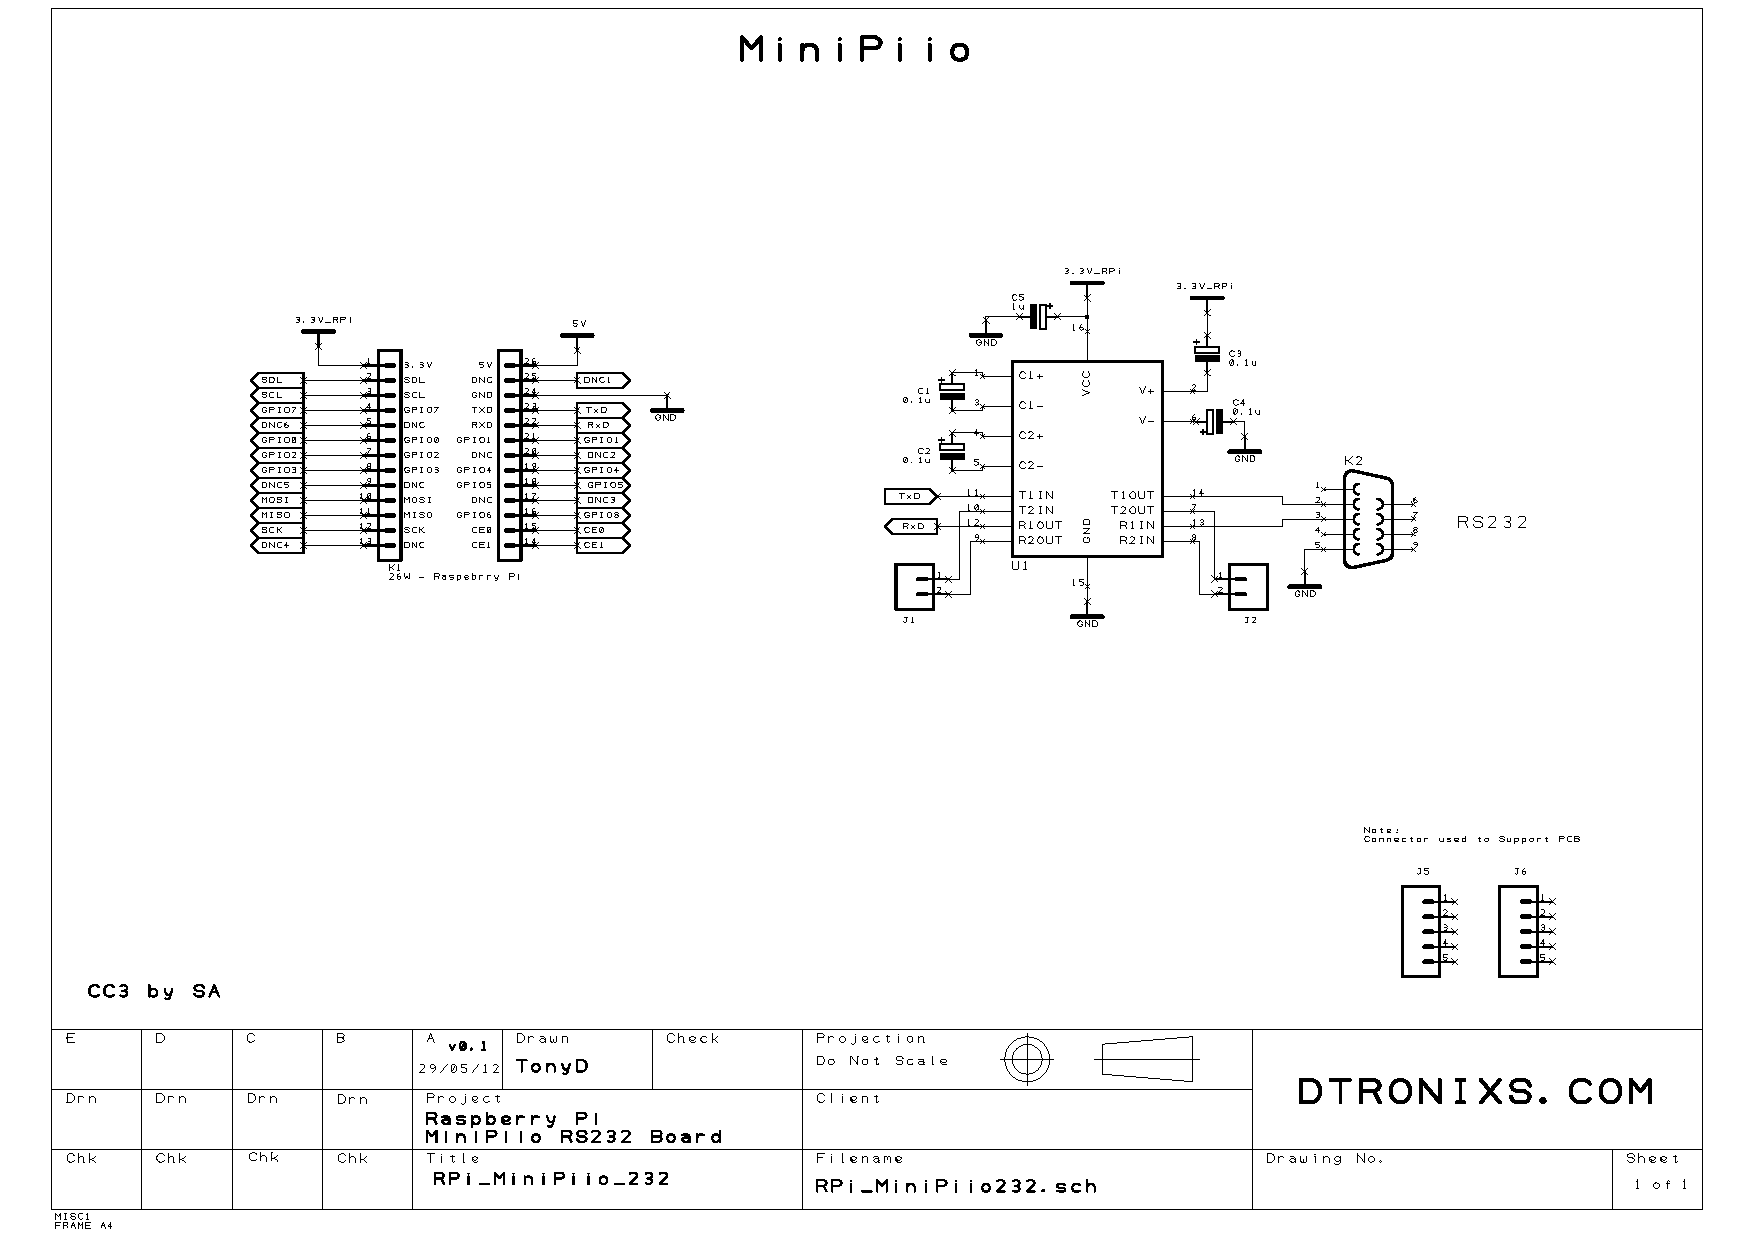
\includegraphics[width=0.7\textwidth, trim=400 250 100 100, clip=true]{../Schematics/UART-to-RS232.pdf}
	\end{center}
	\caption{Schematics for the RS232-converter}
	\label{fig:UART-RS232}
\end{figure}